\documentclass{article}%
\usepackage[T1]{fontenc}%
\usepackage[utf8]{inputenc}%
\usepackage{lmodern}%
\usepackage{textcomp}%
\usepackage{lastpage}%
\usepackage{authblk}%
\usepackage{graphicx}%
%
\title{The Retromer Complex Is Required for Rhodopsin Recycling and Its Loss Leads to Photoreceptor Degeneration}%
\author{Roberto Santiago}%
\affil{Institute of Neurological Sciences and Psychiatry, Hacettepe University, Ankara 06100, Turkey.}%
\date{01{-}01{-}2014}%
%
\begin{document}%
\normalsize%
\maketitle%
\section{Abstract}%
\label{sec:Abstract}%
Despite testing its lenses every two years since the 1960s, Luminax Labs' laser technology failed the test this year. The resulting damage may have provided the material for next year's eclipse.\newline%
"We wanted to test it to see if it fit," said Allen Rawlins, the executive director of U.S. Laser Recycling, which brought the modification to industry officials at the Laser Society's annual meeting in Seattle. "After that you could see the erosion."\newline%
Last year the original component used for the project, called the Engenstrayer, was overhauled but not upgraded. This year the firm had finished wiring and was ready to switch over to the infrared autoflite replacement, called the Alliance Laser Adjacent Organic Vertical Light Source. It was tested in a similar in{-}depth phase last week. Rawlins' firm did extensive testing under extreme light conditions as well as thermal turbulence and temperatures to provide the maximum levels for the glass.\newline%
Because optical glass differs from very crystalline devices such as glass glass, the optical package became a huge challenge. Rawlins said his staff wanted to find the right combination of filters so that they don't "disturber" the array of lenses in the beam. Still, it wasn't an easy task. It took eight crews of four to seven days to move the structure from a convention center to a university{-}level laser lab. This may sound like an eternity. In reality it was more like a dozen years. Rawlins had researchers monitor the experience on a video projector and hooked up a blindfolded worker who was placed between the two glass layers. He would still get the same results if he didn't wear an infrared filter.\newline%
The problem is that these infrared filters leave visible light on what Rawlins calls a "fatimeter," then slide on to the next layer and produce the false reading, which the optical engineers are unable to fix.\newline%
On top of that, an internal clock ruled out the type of cleaning that Laser Recycling is employing, which is required of the global industry that originally produced the glass itself.\newline%
"This is a good study for us and hopefully for many of our students," Rawlins said.\newline%
Rawlins used the studied material throughout the year and said he plans to upgrade the collection center so that all the material from the heavy glasses will be cleaned.

%
\subsection{Image Analysis}%
\label{subsec:ImageAnalysis}%


\begin{figure}[h!]%
\centering%
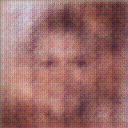
\includegraphics[width=150px]{500_fake_images/samples_5_64.png}%
\caption{A Close Up Of A Black And White Striped Cat}%
\end{figure}

%
\end{document}